\documentclass[aspectratio=169,10pt]{beamer}
\usetheme{metropolis}
\usepackage{booktabs}
\usepackage{amsmath}
\graphicspath{{../figures/}}
\setbeamertemplate{frame footer}{Inventory Demand Forecasting --- Phase 2}
\newcommand{\who}[1]{\hfill{\small\color{gray}Presenter: #1}}

\title{Inventory Demand Forecasting via Kalman Filtering\\and Global DeepAR Models}
\subtitle{Phase 2 --- Deep Learning Evaluation (CSA332)}
\author{Saumya \and Harshvardhan \and Shivansh \and Krishiv \and Harsha}
\date{}

\begin{document}

\maketitle

%---------------------------------------------------------------- 2
\begin{frame}{Problem and plan \who{all}}
\begin{columns}[T]
\column{0.5\textwidth}
\textbf{Task:} forecast 28 days of daily unit sales for 300 Walmart SKUs (M5), with \alert{quantiles}, not only a point.

\medskip
\textbf{Difficulties}
\begin{itemize}
\item most SKUs are intermittent (many zeros)
\item zeros can be \alert{stockouts} (censored demand)
\item new SKUs have almost no history (\alert{cold start})
\end{itemize}
\column{0.5\textwidth}
\textbf{Models compared (same protocol)}
\begin{itemize}
\item Phase 1: seasonal naive, LightGBM, \textbf{Kalman filter} (local)
\item Phase 2: \textbf{DeepAR} (global LSTM, NB likelihood)
\item Phase 2 hybrid: \textbf{KF-DeepAR}
\end{itemize}
\medskip
\textbf{Roles} (random): Saumya data · Harshvardhan Kalman · Shivansh DeepAR · Krishiv hybrid · Harsha evaluation
\end{columns}
\end{frame}

%---------------------------------------------------------------- 3
\begin{frame}{Data: M5 subset and demand segments \who{Saumya}}
\begin{columns}[T]
\column{0.38\textwidth}
\begin{itemize}
\item Store CA\_1; FOODS\_3, HOUSEHOLD\_1, HOBBIES\_1; 100 random SKUs each
\item last 1000 days, complete (SKU $\times$ day) index
\item no price $\Rightarrow$ not on sale $\Rightarrow$ \texttt{NaN}, not 0
\item 201/300 SKUs \alert{intermittent}, 50 lumpy
\item 3 rolling origins, horizon 28
\end{itemize}
\column{0.62\textwidth}
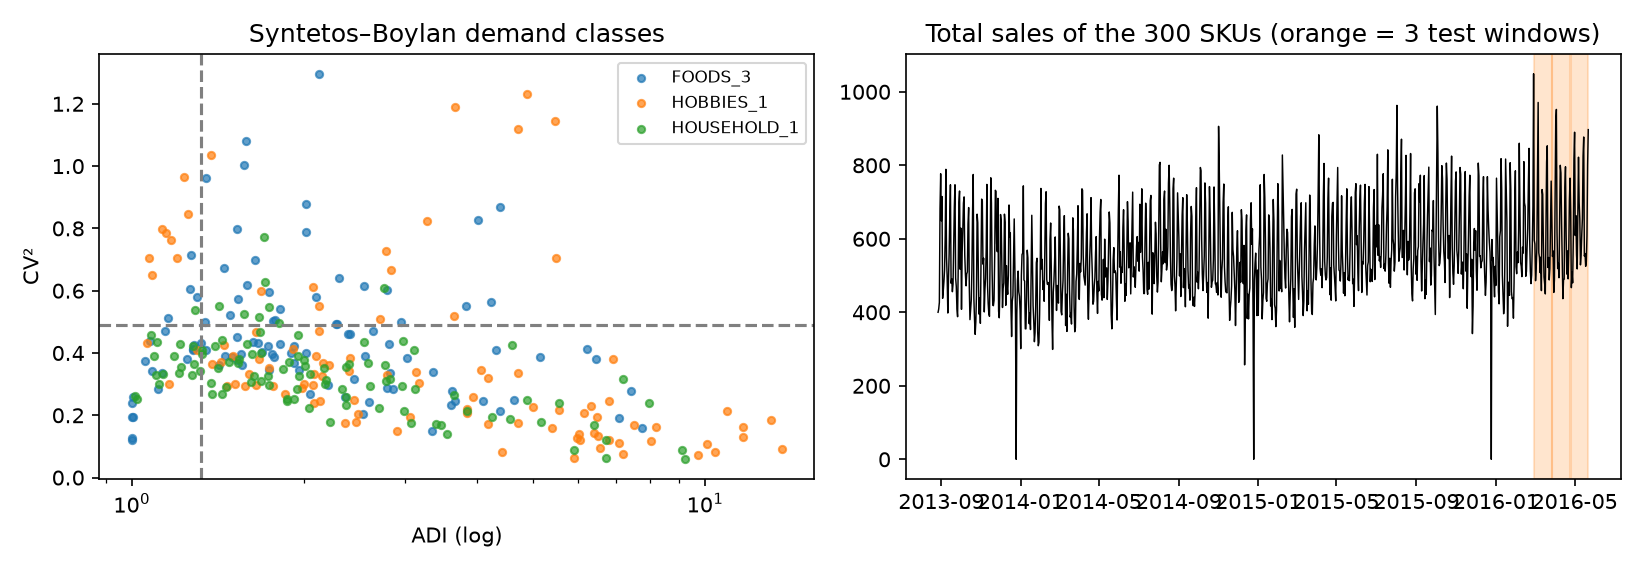
\includegraphics[width=\textwidth]{01_segments_and_total.png}
\end{columns}
\end{frame}

%---------------------------------------------------------------- 4
\begin{frame}{Mark, don't impute --- and the DL windows \who{Saumya}}
\begin{columns}[T]
\column{0.5\textwidth}
\textbf{Causal stockout detector}\\
Poisson rate $\lambda$ from 56 days before a zero-run: flag once $e^{-\lambda k}<10^{-3}$.\\
Uses only $y_{1:t}$ (tested) $\Rightarrow$ 8.6\% of days flagged.
\begin{itemize}
\item excluded from the training loss
\item skipped by the Kalman update
\item reported separately in evaluation
\end{itemize}
\column{0.5\textwidth}
\textbf{DL window} = 56-day context + 28-day prediction\\
\begin{itemize}
\item input at $t$: $y_{t-1}/\nu$ (never $y_t$), 14 known covariates
\item scale $\nu = 1+\text{mean(context)}$
\item random windows each epoch (augmentation)
\end{itemize}
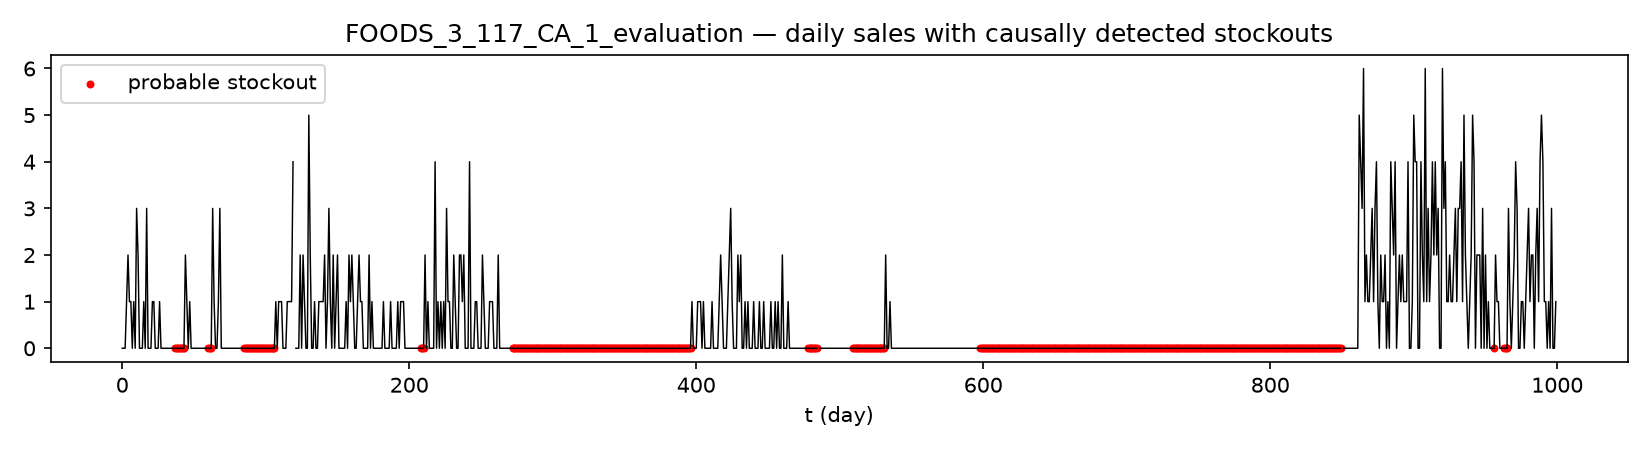
\includegraphics[width=\textwidth]{01_stockout_example.png}
\end{columns}
\end{frame}

%---------------------------------------------------------------- 5
\begin{frame}{Local state: the Kalman filter \who{Harshvardhan}}
\begin{columns}[T]
\column{0.5\textwidth}
$z_t = y_t/s_{dow}$, \quad $x_t=x_{t-1}+w_t$, \quad $z_t=x_t+v_t$
\begin{align*}
P^-_t &= P_{t-1}+q\\
K_t &= P^-_t/(P^-_t+r)\\
\hat x_t &= \hat x_{t-1}+K_t(z_t-\hat x_{t-1})\\
P_t &= (1-K_t)P^-_t
\end{align*}
\begin{itemize}
\item $\rho=q/r$ by maximum likelihood (prediction-error decomposition)
\item missing / stockout day $\Rightarrow$ predict only
\item forecast variance $s^2(P+hq+r)$
\end{itemize}
\column{0.5\textwidth}
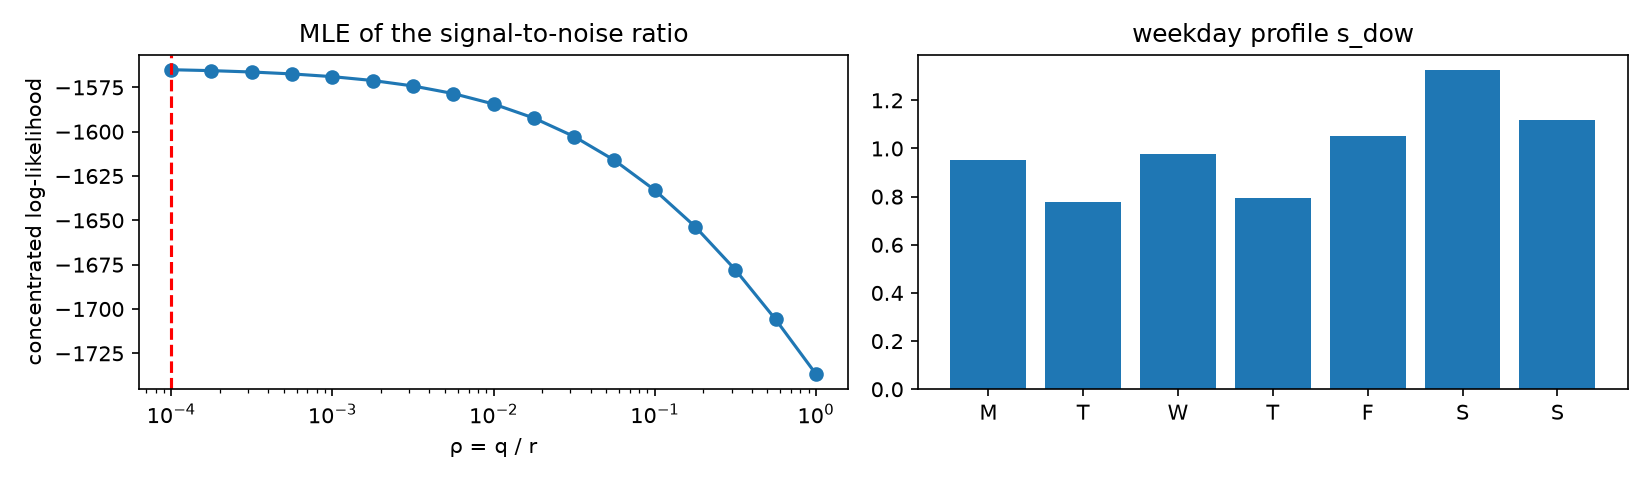
\includegraphics[width=\textwidth]{02_kalman_mle.png}\\
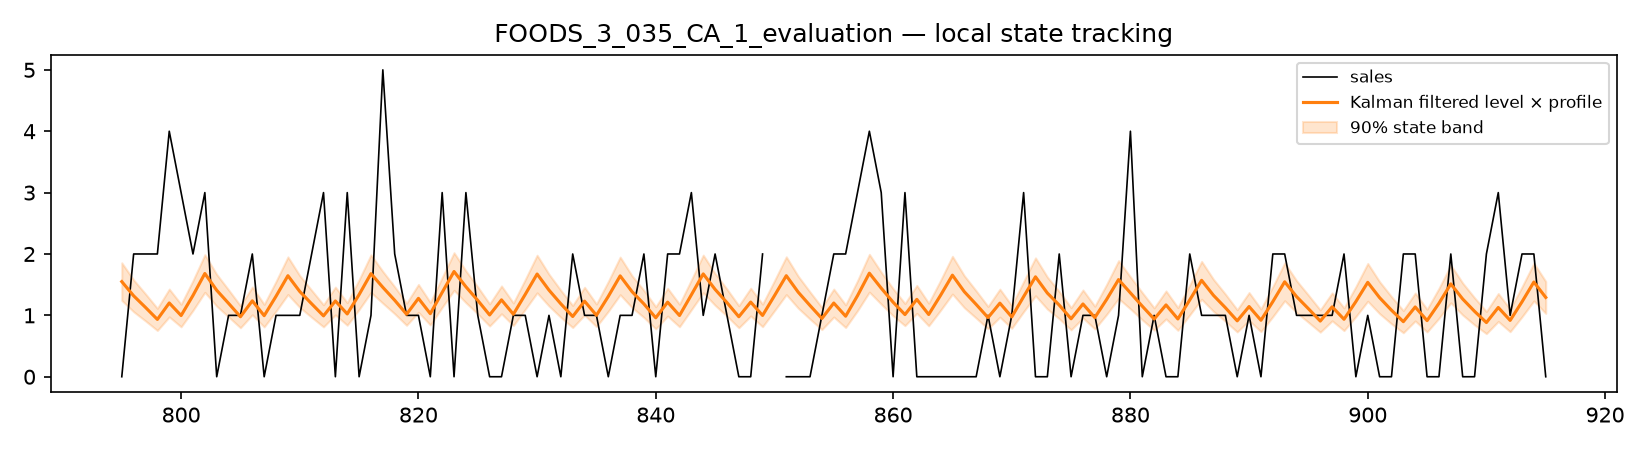
\includegraphics[width=\textwidth]{02_kalman_tracking.png}
\end{columns}
\end{frame}

%---------------------------------------------------------------- 6
\begin{frame}{Phase-1 baselines and the gap \who{Harshvardhan}}
\begin{columns}[T]
\column{0.48\textwidth}
\begin{tabular}{lcc}
\toprule
& WAPE & Pinball\\
\midrule
Seasonal naive & 0.757 & 0.514\\
LightGBM & 0.655 & \textbf{0.402}\\
Kalman & \textbf{0.636} & 0.416\\
\bottomrule
\end{tabular}

\medskip
\textbf{Gap test:} weekday profile from the SKU alone vs.\ pooled over its department.
\begin{itemize}
\item full history: no difference
\item \alert{last 8 weeks only: pooling wins in every segment} (up to +1.8\%)
\end{itemize}
$\Rightarrow$ sparse histories need information from \emph{other} SKUs.
\column{0.52\textwidth}
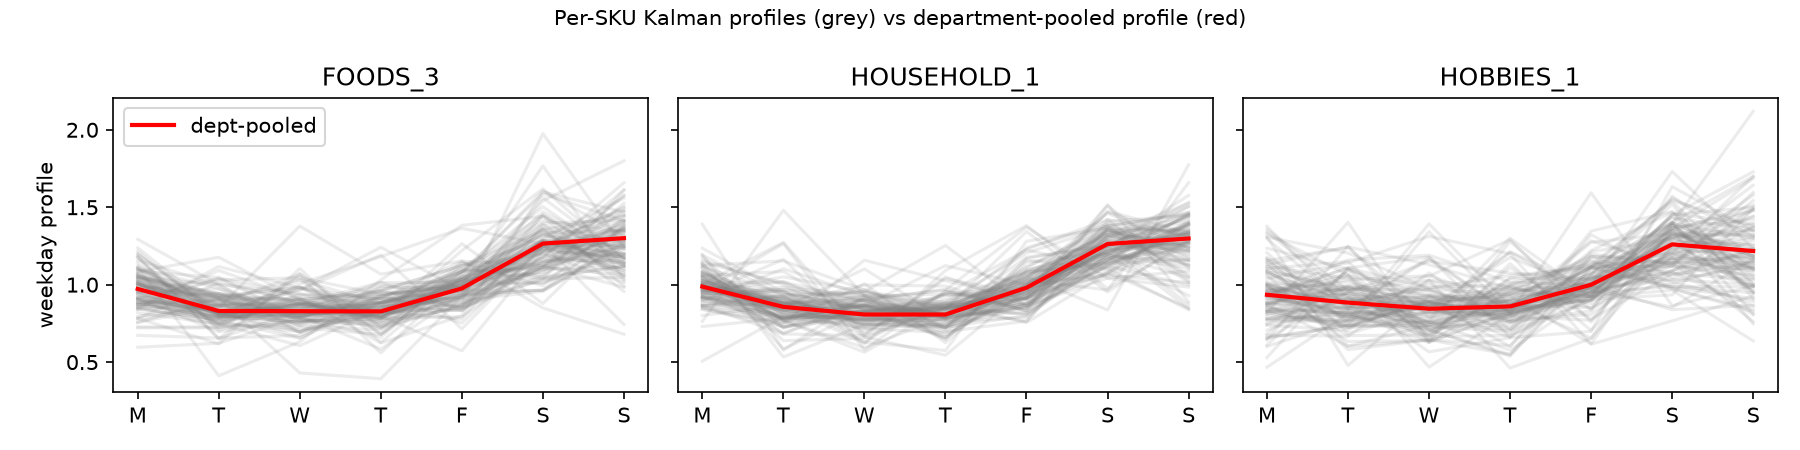
\includegraphics[width=\textwidth]{02_profiles_gap.png}
\end{columns}
\end{frame}

%---------------------------------------------------------------- 7
\begin{frame}{Global DL: DeepAR architecture \who{Shivansh}}
\begin{columns}[T]
\column{0.55\textwidth}
One LSTM (2$\times$40, 27.6k params) for \alert{all} SKUs:
\[ h_t=\text{LSTM}(h_{t-1},[y_{t-1}/\nu,\ \mathbf x_t,\ \mathbf e_{item},\ \mathbf e_{dept}]) \]
Negative Binomial output:
\[ \mu_t=\nu\,\text{softplus}(\cdot),\quad \alpha_t=\text{softplus}(\cdot)/\sqrt\nu \]
mean $\mu$, variance $\mu+\alpha\mu^2$ (counts, over-dispersion)
\begin{itemize}
\item training: masked NLL, teacher forcing
\item forecast: 200 sampled paths $\Rightarrow$ mean, q10/q50/q90
\item LSTM: additive cell update $\Rightarrow$ no vanishing gradient
\end{itemize}
\column{0.45\textwidth}
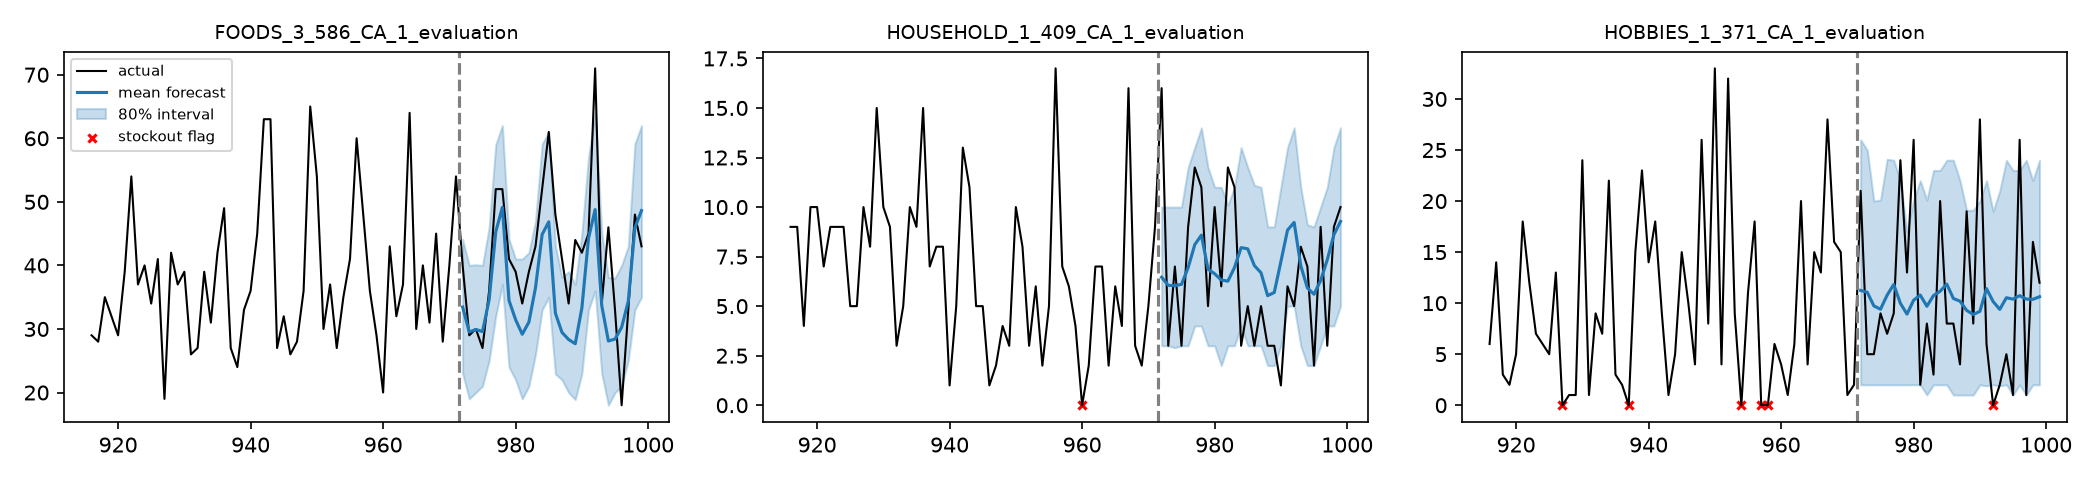
\includegraphics[width=\textwidth]{03_fan_charts.png}\\[2mm]
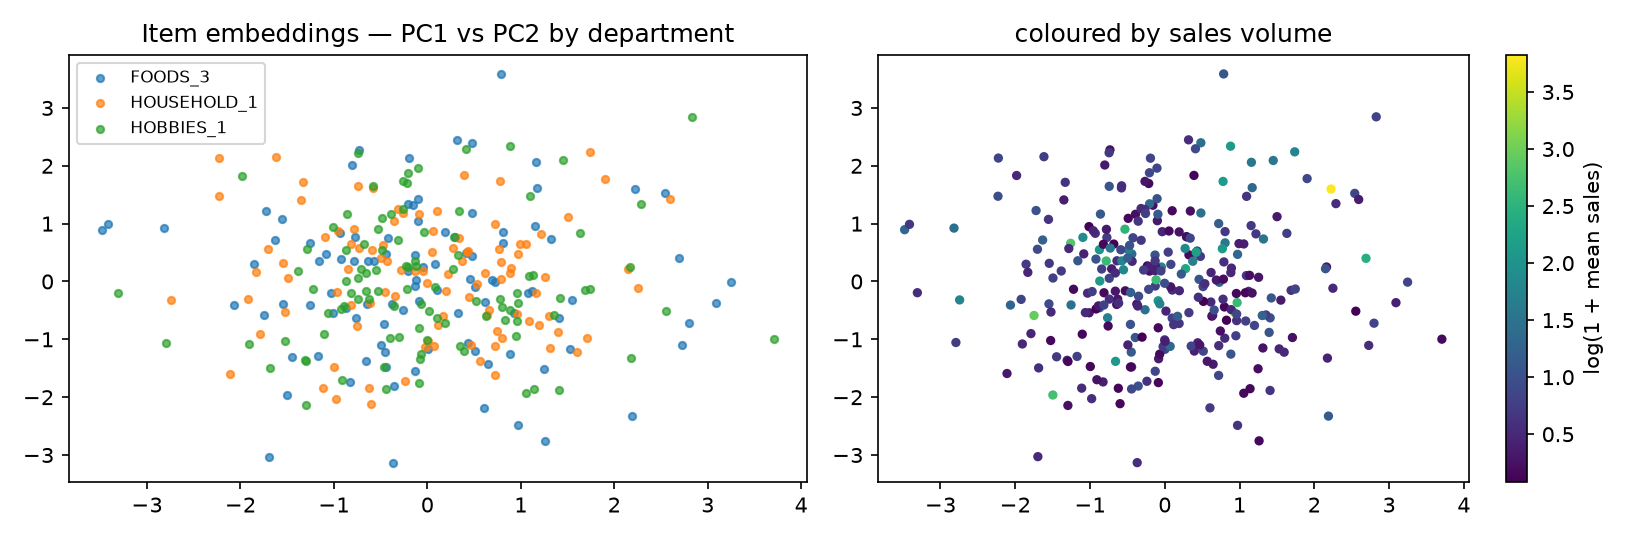
\includegraphics[width=\textwidth]{03_embedding_pca.png}
\end{columns}
\end{frame}

%---------------------------------------------------------------- 8
\begin{frame}{DeepAR: regularisation and results \who{Shivansh}}
\begin{columns}[T]
\column{0.5\textwidth}
\textbf{Regularisation}
\begin{itemize}
\item dropout 0.1, AdamW weight decay $10^{-4}$
\item \alert{item-ID dropout} 0.1 (enables cold start)
\item early stopping on the 28 days before the origin
\item LR halved on plateau, gradient clipping 10
\end{itemize}
\textbf{Result} (3 origins $\times$ 3 seeds)\\
pinball \textbf{0.395 $\pm$ 0.004}\\
$-1.8\%$ vs LightGBM, $-5.1\%$ vs Kalman
\column{0.5\textwidth}
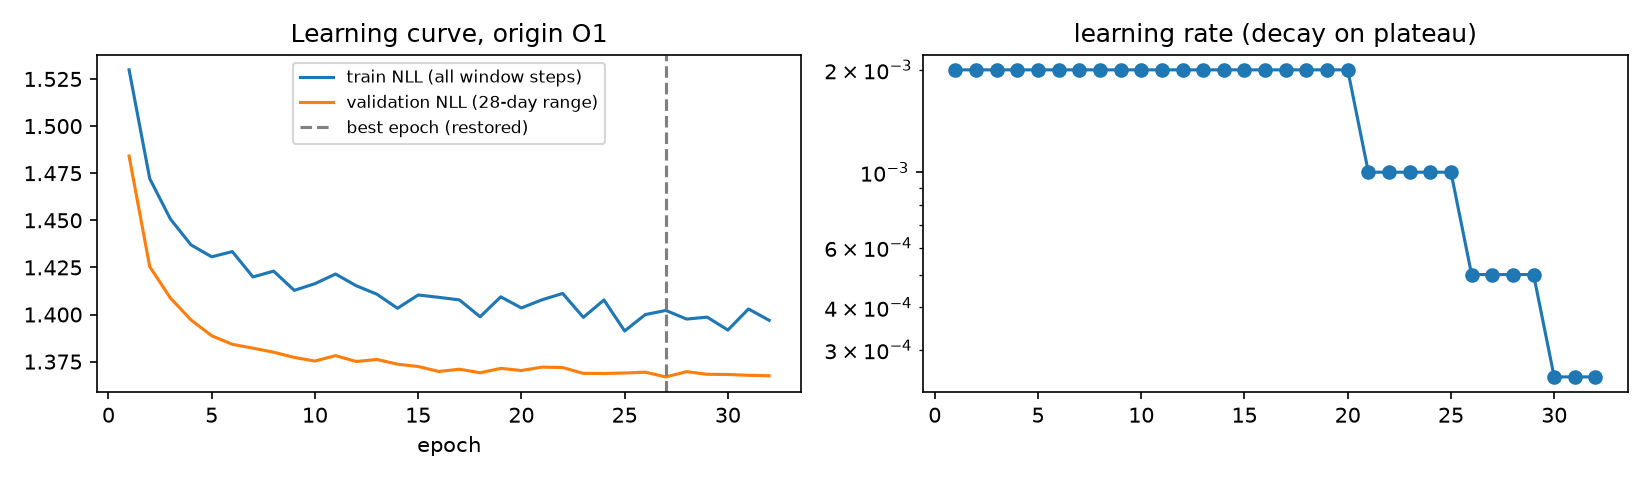
\includegraphics[width=\textwidth]{03_learning_curve.png}
\end{columns}
\end{frame}

%---------------------------------------------------------------- 9
\begin{frame}{Hybrid: Kalman-informed DeepAR (KF-DeepAR) \who{Krishiv}}
\begin{columns}[T]
\column{0.5\textwidth}
\begin{tabular}{lcc}
\toprule
& Kalman & DeepAR\\
\midrule
memory & whole history & 56 days\\
level shift & instant & slow\\
shares patterns & no & yes\\
\bottomrule
\end{tabular}

\medskip
\textbf{Idea:} give DeepAR 2 extra inputs per day --- what the Kalman filter predicts and its std, computed \alert{causally}.\\
The LSTM \emph{learns} when to trust the local state.\\
Family: ES-RNN (M4 winner), Deep State Space Models.
\column{0.5\textwidth}
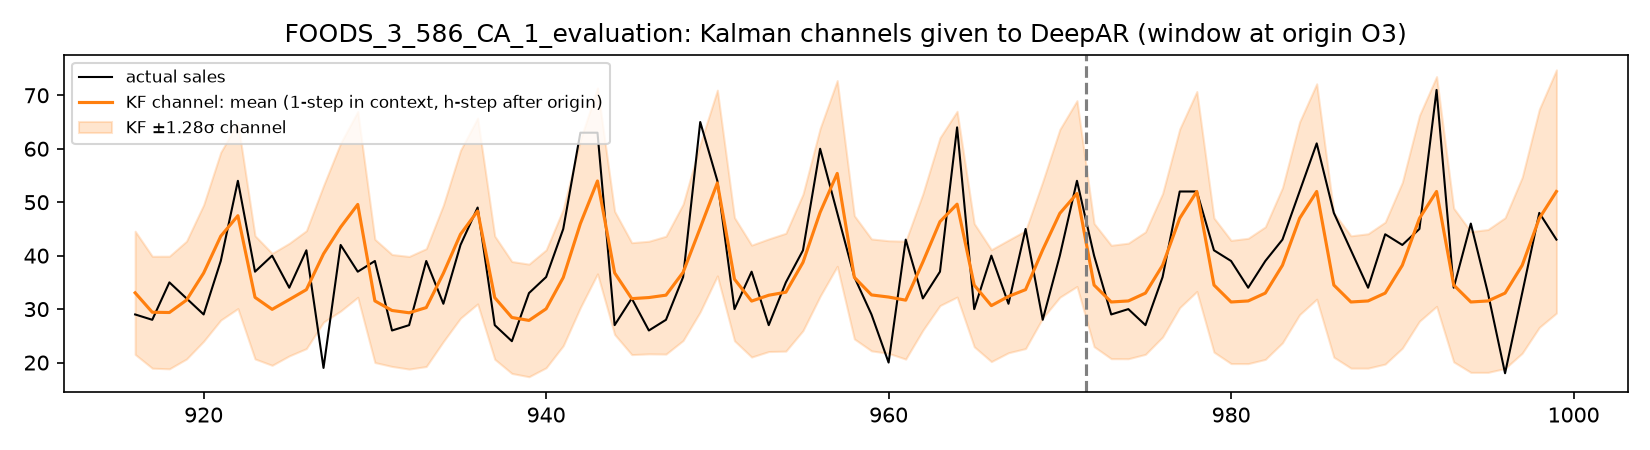
\includegraphics[width=\textwidth]{04_kf_channels.png}
\end{columns}
\end{frame}

%---------------------------------------------------------------- 10
\begin{frame}{Hybrid: results and cold start \who{Krishiv}}
\begin{columns}[T]
\column{0.5\textwidth}
\begin{tabular}{lcc}
\toprule
& Pinball & seed std\\
\midrule
DeepAR & 0.395 & 0.0036\\
50/50 average & 0.400 & 0.0015\\
\textbf{KF-DeepAR} & \textbf{0.394} & \textbf{0.0011}\\
\bottomrule
\end{tabular}
\begin{itemize}
\item significantly better than 50/50 average, LightGBM, Kalman
\item tie with DeepAR (CI contains 0), lower seed variance
\end{itemize}
\column{0.5\textwidth}
\textbf{Cold start} (30 unseen SKUs, 28 days of history)\\[1mm]
\begin{tabular}{lcc}
\toprule
& WAPE & Pinball\\
\midrule
Kalman & 0.615 & 0.571\\
DeepAR & 0.629 & 0.556\\
\textbf{KF-DeepAR} & \textbf{0.612} & \textbf{0.552}\\
\bottomrule
\end{tabular}

\medskip
Hybrid is best when local history is scarce.
\end{columns}
\end{frame}

%---------------------------------------------------------------- 11
\begin{frame}{Evaluation protocol \who{Harsha}}
\begin{itemize}
\item \textbf{Rolling origins} O1--O3: train $\le o-28$, validate $(o-28,o]$, test $(o,o+28]$; refit per origin
\item \textbf{Same cells, same horizons} for every model (25{,}200 test cells)
\item \textbf{Metrics}: MAE, RMSE, WAPE (mean forecast); pinball loss over $\tau\in\{0.1,0.5,0.9\}$; 80\% coverage and width
\item \textbf{Pinball} $L_\tau=\max(\tau(y-q),(\tau-1)(y-q))$ is a \alert{strictly proper} scoring rule
\item \textbf{3 seeds} per deep model; paired bootstrap over SKUs for significance
\item metrics on all days \emph{and} on in-stock days only
\end{itemize}
\end{frame}

%---------------------------------------------------------------- 12
\begin{frame}{Final rolling-origin report \who{Harsha}}
\begin{columns}[T]
\column{0.52\textwidth}
\small
\begin{tabular}{lccc}
\toprule
Model & WAPE & Pinball & Cov80\\
\midrule
Seasonal naive & 0.757 & 0.514 & 0.84\\
LightGBM & 0.655 & 0.402 & 0.80\\
Kalman & 0.636 & 0.416 & 0.87\\
DeepAR & 0.641 & 0.395 & 0.91\\
50/50 avg & \textbf{0.633} & 0.400 & 0.86\\
\textbf{KF-DeepAR} & 0.641 & \textbf{0.394} & 0.91\\
\bottomrule
\end{tabular}

\medskip
Deep models win most on \alert{lumpy} SKUs ($-9.6\%$ pinball vs Kalman).
\column{0.48\textwidth}
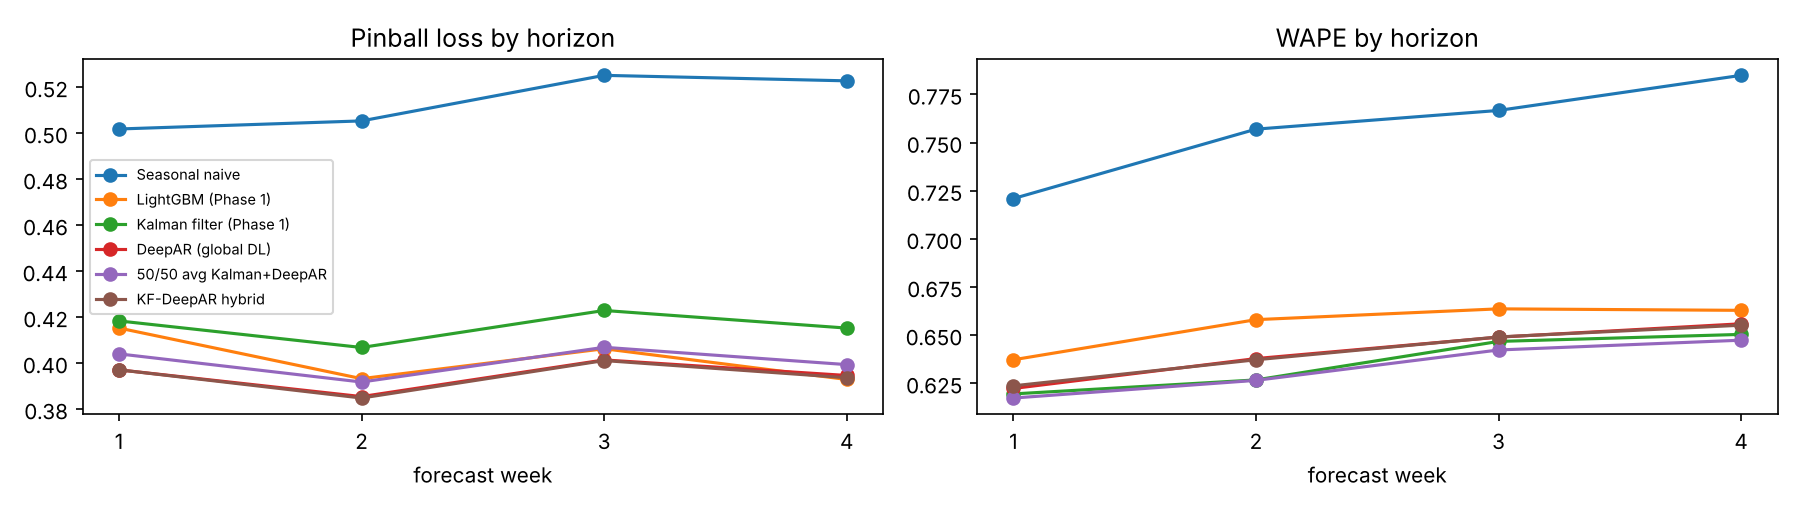
\includegraphics[width=\textwidth]{06_by_horizon.png}\\
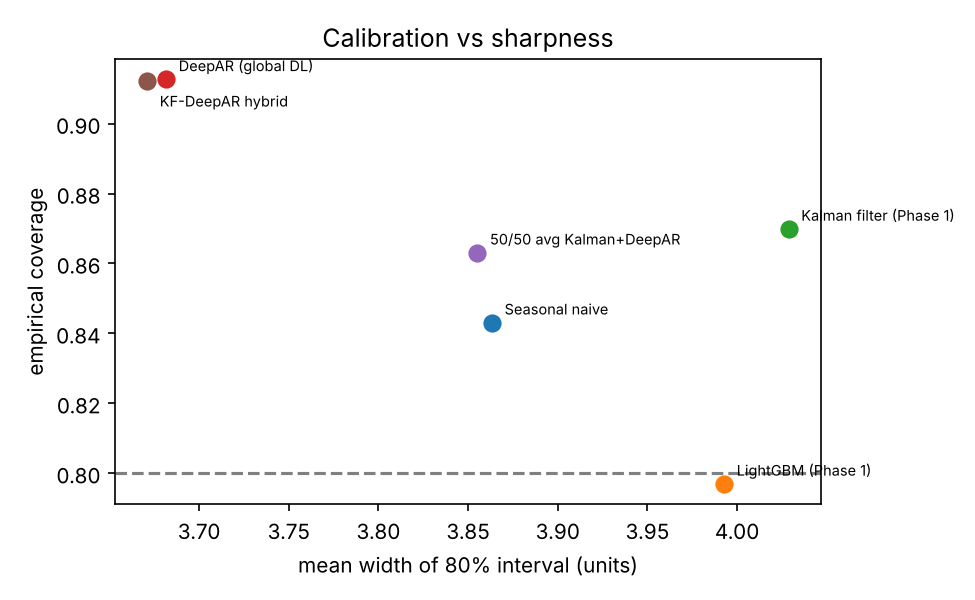
\includegraphics[width=0.75\textwidth]{06_coverage_width.png}
\end{columns}
\end{frame}

%---------------------------------------------------------------- 13
\begin{frame}{Ablation study (3 origins $\times$ 3 seeds) \who{Harsha}}
\begin{columns}[T]
\column{0.5\textwidth}
\small
\begin{tabular}{lcc}
\toprule
Remove / change & $\Delta$ pinball & worse\\
\midrule
A1 Kalman channels & +0.1\% & 5/9\\
A2 item embedding & +0.4\% & 4/9\\
A3 calendar \& price & 0.0\% & 4/9\\
\alert{A4 Gaussian likelihood} & \alert{+4.8\%} & \alert{9/9}\\
A5 GRU for LSTM & 0.0\% & 3/9\\
A6 regularisation & $-$0.1\% & 5/9\\
A7 stockout masking & $-$0.9\%$^*$ & 2/9\\
\bottomrule
\end{tabular}

\smallskip
{\footnotesize $^*$ on in-stock days only $-0.1\%$: it only ``wins'' by predicting censored zeros.}
\column{0.5\textwidth}
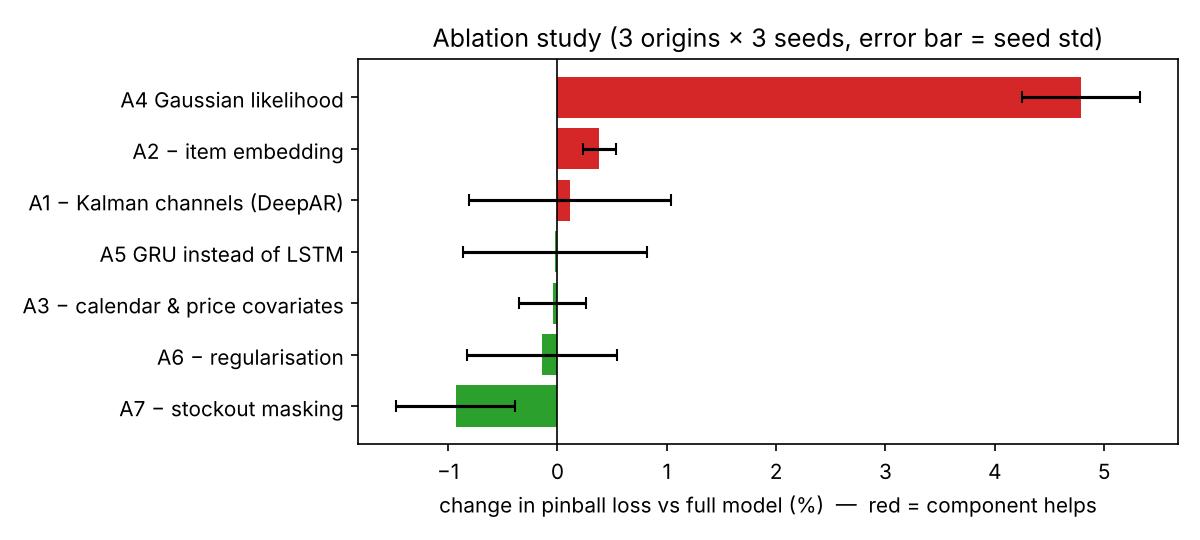
\includegraphics[width=\textwidth]{05_ablation_bar.png}
\begin{itemize}\small
\item the \alert{count likelihood} is what matters
\item other choices are within seed noise
\end{itemize}
\end{columns}
\end{frame}

%---------------------------------------------------------------- 14
\begin{frame}{Discussion and limitations \who{all}}
\begin{itemize}
\item Kalman: strong point forecasts, weak distributions and sparse series
\item Global DL: better probabilistic accuracy, especially intermittent / lumpy SKUs
\item Hybrid: meaningful where local information is scarce (cold start); small average gain because most filters are very smooth ($q/r\approx 6\cdot 10^{-4}$)
\item Ablations: the NB likelihood matters most; LSTM vs GRU and regularisation are within seed noise
\item Limitations: one store, 300 SKUs; heuristic stockout flags; no hyper-parameter tuning; discrete data inflates coverage
\end{itemize}
\end{frame}

%---------------------------------------------------------------- 15
\begin{frame}{Conclusion and future work \who{all}}
\begin{itemize}
\item Leak-free DL pipeline, from-scratch DeepAR, Kalman-informed hybrid, full rolling-origin report with uncertainty
\item Global DL beats local and tabular baselines on pinball loss; the hybrid has the lowest pinball loss and is best at cold start
\item Next: network outputs the Kalman noise per SKU and day (deep state-space model); attention (TFT) or selective SSM (Mamba) encoder; tune the stockout threshold
\end{itemize}
\vfill
\centering Thank you --- questions?
\end{frame}

\end{document}
